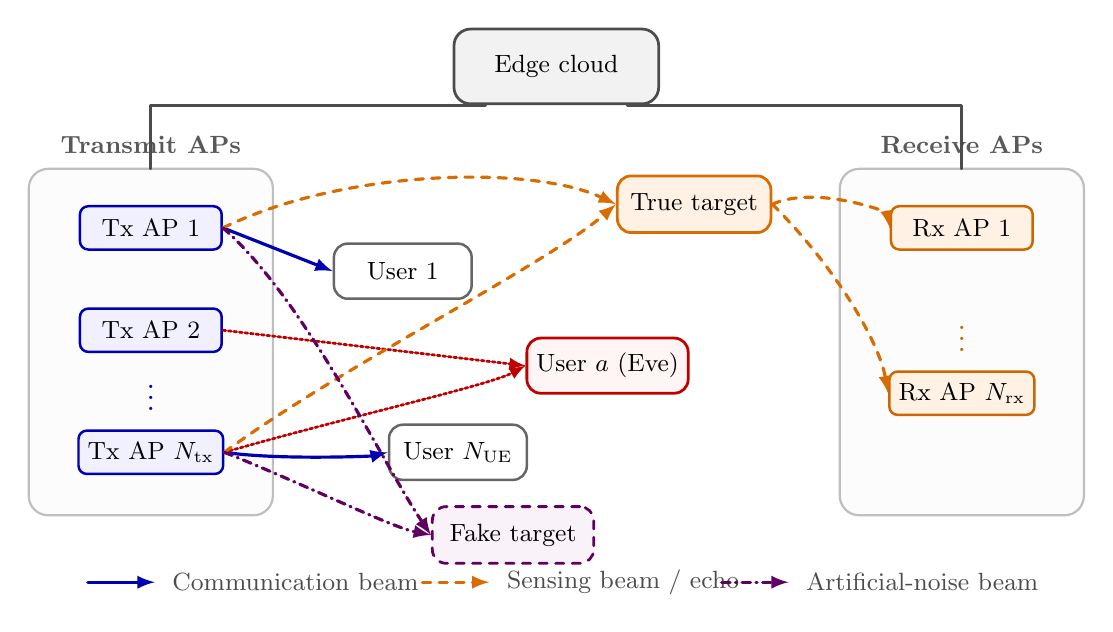
\begin{tikzpicture}[x=1cm,y=1cm,>=latex,font=\small,line cap=round,line join=round]
\colorlet{txc}{blue!70!black}
\colorlet{rxc}{orange!80!black}
\colorlet{sensc}{orange!85!black}
\colorlet{evec}{red!75!black}
\colorlet{anc}{violet!75!black}
\colorlet{cloudc}{black!70}

\tikzset{
panel/.style={draw=black!25, rounded corners=7pt, line width=0.8pt, fill=black!1},
cloudbox/.style={draw=cloudc, rounded corners=6pt, line width=1pt, fill=gray!10, minimum width=2.6cm, minimum height=0.95cm},
txnode/.style={draw=txc, rounded corners=3pt, line width=0.9pt, fill=blue!6, minimum width=1.8cm, minimum height=0.55cm},
rxnode/.style={draw=rxc, rounded corners=3pt, line width=0.9pt, fill=orange!10, minimum width=1.8cm, minimum height=0.55cm},
usernode/.style={draw=black!60, rounded corners=5pt, line width=0.9pt, fill=white, minimum width=1.75cm, minimum height=0.7cm},
evenode/.style={draw=evec, rounded corners=5pt, line width=1pt, fill=red!4, minimum width=2.0cm, minimum height=0.7cm},
targetnode/.style={draw=sensc, rounded corners=5pt, line width=1pt, fill=orange!10, minimum width=1.95cm, minimum height=0.72cm},
fakenode/.style={draw=anc, rounded corners=5pt, line width=1pt, dashed, fill=violet!5, minimum width=2.05cm, minimum height=0.72cm}
}

\node[cloudbox] (cloud) at (0,4.05) {Edge cloud};

\draw[panel] (-6.7,-1.65) rectangle (-3.6,2.75);
\node[text=black!65, font=\small\bfseries] at (-5.15,3.05) {Transmit APs};
\node[txnode] (tx1) at (-5.15,2.00) {Tx AP 1};
\node[txnode] (tx2) at (-5.15,0.70) {Tx AP 2};
\node[text=txc, font=\large] at (-5.15,-0.05) {$\vdots$};
\node[txnode] (txn) at (-5.15,-0.85) {Tx AP $N_{\mathrm{tx}}$};

\draw[panel] (3.6,-1.65) rectangle (6.7,2.75);
\node[text=black!65, font=\small\bfseries] at (5.15,3.05) {Receive APs};
\node[rxnode] (rx1) at (5.15,2.00) {Rx AP 1};
\node[text=rxc, font=\large] at (5.15,0.70) {$\vdots$};
\node[rxnode] (rxn) at (5.15,-0.10) {Rx AP $N_{\mathrm{rx}}$};

\draw[cloudc, line width=1pt] (-0.9,3.55) -- (-5.15,3.55) -- (-5.15,2.75);
\draw[cloudc, line width=1pt] (0.9,3.55) -- (5.15,3.55) -- (5.15,2.75);

\node[usernode] (u1) at (-1.95,1.45) {User 1};
\node[usernode] (un) at (-1.25,-0.85) {User $N_{\mathrm{UE}}$};
\node[evenode] (eve) at (0.65,0.25) {User $a$ (Eve)};
\node[targetnode] (target) at (1.75,2.30) {True target};
\node[fakenode] (fake) at (-0.55,-1.90) {Fake target};

\draw[txc, line width=1.15pt, -latex] (tx1.east) -- (u1.west);
\draw[txc, line width=1.15pt, -latex] (txn.east) .. controls (-3.55,-0.95) and (-2.35,-0.90) .. (un.west);
\draw[evec, densely dotted, line width=1pt, -latex] (tx2.east) -- (eve.west);
\draw[evec, densely dotted, line width=1pt, -latex] (txn.east) .. controls (-2.65,-0.40) and (-0.85,0.00) .. (eve.west);

\draw[sensc, dashed, line width=1.15pt, -latex] (tx1.east) .. controls (-2.70,2.75) and (-0.30,2.80) .. (target.west);
\draw[sensc, dashed, line width=1.15pt, -latex] (txn.east) .. controls (-2.80,0.20) and (-0.10,1.55) .. (target.west);
\draw[sensc, dashed, line width=1.15pt, -latex] (target.east) .. controls (3.30,2.55) and (4.20,2.20) .. (rx1.west);
\draw[sensc, dashed, line width=1.15pt, -latex] (target.east) .. controls (3.55,1.50) and (4.10,0.55) .. (rxn.west);

\draw[anc, dash dot, line width=1.15pt, -latex] (tx1.east) .. controls (-3.20,1.10) and (-2.20,-1.00) .. (fake.west);
\draw[anc, dash dot, line width=1.15pt, -latex] (txn.east) .. controls (-3.10,-1.30) and (-2.10,-1.80) .. (fake.west);


\draw[txc, line width=1.15pt, -latex] (-5.95,-2.50) -- (-5.10,-2.50);
\node[anchor=west, text=black!70] at (-5.00,-2.50) {Communication beam};
\draw[sensc, dashed, line width=1.15pt, -latex] (-1.70,-2.50) -- (-0.85,-2.50);
\node[anchor=west, text=black!70] at (-0.75,-2.50) {Sensing beam / echo};
\draw[anc, dash dot, line width=1.15pt, -latex] (2.10,-2.50) -- (2.95,-2.50);
\node[anchor=west, text=black!70] at (3.05,-2.50) {Artificial-noise beam};
\end{tikzpicture}